\chapter{Introduction}
\label{chapter1}



This chapter introduces the related literature review, motivation and goals of the undertaken research.
The chapter begins with a brief preface of cryptology and its importance in the era Internet of Things (IoT) and Big Data.
In \secref{ch1_subsec_pkc} we present how Public-Key Cryptography (PKC) is shaping the security of our every day life.
We introduce the importance of Pairing-Based Cryptography(PBC) in \secref{ch1_subsec_pbc} for the next generation of security protocols. 
\secref{ch1_sec_motivation} presents the motivation behind the works undertaken to assemble of this thesis.
\secref{ch1_sec_outline} outlines the overall organization of this thesis.

\section{Cryptology}
\label{ch1_sec_crypto}
Cryptography is the science of communicating with the authentic receiver through an insecure channel in secret. 
Cryptanalysis is the techniques of breaking the secret communications.
Cryptology is the combination of these two domains.

The history of Cryptography dates back to the time of the Greek and Roman empire.
Julius Caesar used a simple shift and substitute system.
Up until the early '70s of the last century, cryptology was evolved mostly for military purposes. 
The cryptography got its first democratic form in 1975 when Diffie and Hellman invented the concept of public-key cryptography \cite{diffie1976new}. 
The concept was first realized by as practical cryptosystem by the works of Rivest, Shamir and Adleman (RSA) in 1977 \cite{rivest1978method}.
At the same time in 1977, National Bureau of Standards published a cryptosystem intended for the governmental agencies or banks with the named Data Encryption Standard (DES).
From then a new era of cryptography known as \textit{Modern cryptography} was initiated.
The well-organized procedures called \textit{protocols} is the basis of Modern cryptography.
One of the most elegant features of modern crypto-protocols is their inner algorithms are not secret yet withstand cryptanalysis from experts/attackers.
More importantly, these protocols are easy to use for people with no understanding of the underlying principles.
For example, paying by credit cards or withdrawing money using debit cards with a personal identification number (PIN) is doable without concerning what’s going on under the hood. 

The little basic functionality of modern cryptosystem is to enable a sender (Alice \footnote{Alice and Bob are fictional characters first used by Rivest, Shamir and Adleman in \cite{rivest1978method} as placeholder name in cryptology.}) to convert a message (plaintext) into a cipher (ciphertext) before sending to a legitimate receiver (Bob) over the public communication media. 
The receiver can convert the cipher back into the original message using secret information named as a key.
An adversary (Eve) eavesdrops in the middle of the conversation to retrieve information from the cipher.
The cipher is safe from to the adversary until the key is not compromised. 

The security of modern cryptosystems depend not on the secrecy of the encryption algorithms but on the difficulty of one way problems. 
Such problems are easy to calculate in one direction but practically impossible to calculate in reverse direction in a reasonable amount of time using reasonable resources.
For example, let us consider a cipher text $\cal{C}$ and a plaintext $\cal{P}$ and a 128-bit key $\cal{K}$. 
The encryption scheme $\cal{E}$ takes input $\cal{P}$ and $\cal{K}$ and output $\cal{C}=E( \cal{P}, K)$. 
To obtain the  key $\cal{K}$ from the $(\cal{P,C})$ pair, we need to try $2^{128} = 340,282,366,920,938,463,463,374,607,431,768,211,456 \approx 3.4 \times 10^{38}$ (39 decimal digits) combination of $128$-bit keys.
The most powerful supercomputer till this date  can compute 122.3 peta ($10^{15}$) floating-point operations per second (PFLOPS).
Let us consider an  optimistic assumption that 1000 (FLOPS) is required to check one key combination.
Under this assumption, the supercomputer can compute $122.3. \times 10^{15} / 1000 = 122.3 \times 10^{12}$ key combinations per second.
Then it will take about $3.4 \times 10^{38}/((122.3 \times 10^{12})(365 \times 24 \times 60 \times 60)) \approx  8.8 \times 10^{16}$ earth years.
According to the standard model of physical cosmology \cite{Ade:2015xua} the age of our universe is $13.8 \time 10^9$ or 13.8 billion years. 
It means finding a key using brute force search will require $6.3$ million years more than the age of the universe.
We can imagine how big the number $2^{128}$ is from this comparison.



Cryptography became more important as individuals and business increasingly depend on the Internet as a channel for communication. Therefore, the following four properties are the basis of a cryptosystem.


\begin{itemize}
\item Data confidentiality:
This property ensures that confidential information such as bank transactions or medical data etc. are secret from unauthorized entities. 

\item Data integrity:
When data is stored, this property ensures that it not only kept secret (Data confidentiality) but also not rigged.
Confidentiality and integrity is enforced by encryption.

\item Authentication:
In a connection-oriented communication authentication proves both parties identity before communication begins.
Digital signature is used for this purpose to sign a message electronically.
It shields the legitimate party against masquerader from impersonating as a trusted party.
This property gives the receiver a confidence to believe that the message sent over the insecure channel is indeed sent by the actual signee.

\item Non-repudiation:
Non-repudiation (with proof of origin and with proof of receipt) ensures that sender and receiver can not deny having taken part in a communication.
This is important for many cases especially e-commerce while communicating over the Internet.
\end{itemize}

The modern crypto-protocols fall in following two major categories. 

\subsection{Symmetric/Private-Key Cryptography}
Private-Key Cryptography, also known Symmetric Cryptography is the technique where both the sender and the receiver use same \textit{key} or easily derivable from one another to encrypt and decrypt a message.
This type of cryptography is very old history. 

Modern cryptosystems offer efficient symmetric cryptography algorithms, e.g Advanced Encryption Standard (AES) \cite{AES_DaemenR02}.
Such cryptography has two main obstacles i.e. \textit{Key management} and \textit{key establishment}.
Since the keys are same, they need to kept private (\textit{Key management})  in both ends and should be shared securely beforehand (\textit{Key establishment}) without physically meeting.

The Public-key Cryptography offers the solution for \textit{Key establishment} applying Diffie-Hellman key exchange.
This work primarily focuses on a certain type of Public-key Cryptography. 
The subsequent chapters will describe in details.

\subsection{Public-key Cryptography}
\label{ch1_subsec_pkc}
The inception of public-key cryptography solved the problem of key distribution of Symmetric-key cryptography.
It is also know as Asymmetric Cryptography.
The basic idea of  public-key cryptography is to use two different keys for each communicating party .
One key is public-key which can be used by anyone to encrypt message. 
The receiver needs correlated private key to decrypt the message.
From a given public key and cipher text it is asymptotically difficult to obtain the private key.

As afore mentioned, In 1976, Whitfield Diffie and Martin Hellman published their monumental work as a key exchange  protocol\cite{diffie1976new}.  
\fgref{fig_DHKE} shows the simple overview of the Diffie-Hellman Key Exchange (DHKE).
The problems of key distribution and storage associated with symmetric cryptography were the motivation behind the concept of Asymmetric Cryptography, also referred to as Public- Key Cryptography. 

In brief, the protocol has two public parameters, prime number $p$ and a generator $g$ known to all the parties involved in the communication.
The main idea is of this protocol is based on the difficulty to solve the one way function i.e. discrete logarithm.
Let's say, it is easy to calculate Alice public key $k_A$ using Alice private key $k_{Ad}$ as $k_A = g^{k_{Ad}} (\bmod ~p).$ 
However, it will be difficult to obtain $k_{Ad}$ from $k_A, g$ and $p$.
In other words, it is easy to calculate the public key from the private key but the reverse process is practically impossible.
Using this key-exchange we change establish a shared secret which can be used for further encrypted communication.

  \begin{figure}
	\centering
	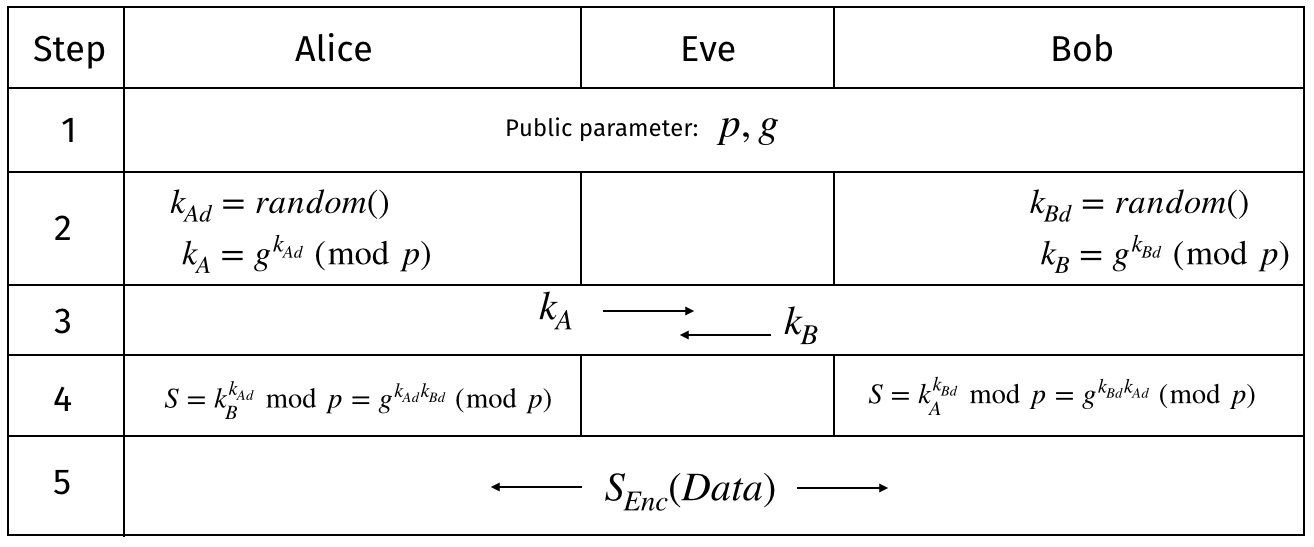
\includegraphics[width=.9\linewidth, height=.67\textheight, keepaspectratio]{Figures/DHKE}
	\caption{Exchanging shared secret key using DH-key exchange.}
	\label{fig_DHKE}
\end{figure}

Rivest, Shamir and Adleman (RSA) realized this protocol in 1977 and published their magnum opus which is widely known as RSA cryptosystem \cite{rivest1978method}. 
The security of the RSA depends on the difficulty of factorization of a larger integer into its two prime factors and the trapdoor permutation for encryption.
Let us denote  two large primes $p$ and $q$ (in practice about 1000-bit).
It is easy to calculate their product to get $n = pq$.
The reverse process that is for a given integer $n$ it will be very difficult to retain $p$ and $q$.
Using the state-of-the art integer factoring algorithm \textit{general number field sieve }(GNFS), it will take appoximately $2^{90}$ basic operation to factor a 2048-bit integer.
After more than 40 year of the RSA breakthrough, it is still standing as an epitome of public key cryptography.
Beside encryption, RSA also enables \textit{digital signature }where the sender uses his private key to sign a message and the receiver verifies the signature by the senders public key. 
Verification of a digitally signed message gives the receiver the confidence that a senders private key is tied to his public key.
It is done to prevent forgery and holds \textit{Non-repudiation} property.

In the mid 80's the independent work of Miller \cite{C:Miller85} and Koblitz \cite{koblitz1987elliptic} began the journey of elliptic curve cryptosystems (ECC). 
The security of  elliptic curve cryptography  protocols depends on the difficulty to solve elliptic curve discrete logarithm problem.
The mathematical details of this problem appears in Chapter 2. %TODO
ECC provides shorter key length for the same level of security than RSA which makes ECC  popular among the researchers. 
Compared to RSA, ECC has other advantages. 
While RSA provides encryption and digital signature; ECC has a family of algorithms for encryption, signature, key agreement and some advanced high-level cryptographic protocols such as ID-based encryption \cite{AC:BonLynSha01} where user's unique ID e.g. email address can be used as a public key. 
The high level cryptographic functionalities are provided by paring over elliptic curves \cite{TODO} which brings a new paradigm in cryptography called pairing-based cryptography.

\subsection{Pairing-Based Cryptography}
\label{ch1_subsec_pbc}
Since the inception by Sakai et al. \cite{sakai2000cryptosystems}, pairing-based cryptography has gained much attention to cryptographic researchers as well as  to mathematicians. It gives flexibility to protocol researcher to innovate applications with provable security and at the same time to mathematicians and cryptography engineers to find efficient algorithms to make pairing implementation more efficient and practical.

Generally, a pairing is a bilinear map $e$ typically defined as  $\g1 \times \g2 \to \g3$, where $\g1$ and $\g2$ are additive cyclic sub-groups of  order $r$  on a certain elliptic curve $E$ over a finite extension field $\FPK$ and $\g3$ is a multiplicative cyclic group of order $r$ in $\mF{p}{k}$.
Let $E(\Fp)$ be the set of rational points over the prime field $\Fp$ which forms an additive Abelian group together with the point at infinity $\cal{O}$. The total number of rational points is denoted as $\#E(\Fp)$. Here, the order $r$ is a large prime number such that $r | \#E(\Fp)$ and gcd$(r,p)=1$. The embedding degree $k$ is the smallest positive integer such that $r | (p^k -1)$.
Two basic properties of pairing are
\begin{itemize}
	\item bilinearity is such that $\forall P_i \in \g1$ and $\forall Q_i \in \g2$, where $i= 1, 2$, then $e(Q_1+Q_2,P_1) = e(Q_1,P_1). e(Q_2,P_1)$ and $e(Q_1,P_1+P_2) = e(Q_1,P_1). e(Q_1,P_2)$,
	\item and $e$ is non-degenerate means $\forall P \in \g1$ there is a $Q \in \g2$ such that  $e(Q,P) \neq 1$ and $\forall Q \in \g2$ there is a $P \in \g1$ such that $e(P,Q) \neq 1$.
\end{itemize}
Such properties allows researchers to come up with various cryptographic applications including ID-based encryption \cite{C:BonFra01}, group signature authentication \cite{C:BonBoySha04}, and functional encryption \cite{C:OkaTak10}.  However, the security of pairing-based cryptosystems depends  on 
\begin{itemize}
	\item  the difficulty of solving elliptic curve discrete logarithm problem (ECDLP) in the groups of order $r$ over $\Fp$,
	\item  the infeasibility of solving the discrete logarithm problem (DLP) in the multiplicative group $\g3 \in \mF{p}{k}$,
	\item and the difficulty of pairing inversion.
\end{itemize}
To maintain the same security level in both groups, the size of the order $r$ and extension field $p^k$ is chosen accordingly. If the desired security level is $\delta$ then $\log_2 r  \geq 2\delta$ is desirable due to Pollard's rho algorithm \cite{TODO}.  For efficient pairing, the ratio $\rho = \log_2 p^k/ \log_2 r \approx 1$,   is expected (usually  $1\leq  \rho  \leq 2$). In practice, elliptic curves with small embedding degrees $k$ and large $r$ are selected and commonly are knows as ``pairing-friendly" elliptic curves.

Galbraith et al. \cite{galbraith2008pairings} have classified pairings as three major categories based on the underlying group's structure as 
\begin{itemize}
	\item Type 1, where $\g1 = \g2$, also known as symmetric pairing. 
	\item Type 2, where $\g1 \neq \g2$, known as asymmetric pairing. There exists an efficiently computable isomorphism $\psi : \g2 \to \g1$ but none in reverse direction.
	\item Type 3, which is also asymmetric pairing, i.e., $\g1 \neq \g2$. But no efficiently computable isomorphism is known in either direction  between $\g1$ and $\g2$.
\end{itemize}




%This thesis chooses one of the Type 3 variants of pairing named as Optimal-Ate \cite{DBLP:journals/tit/Vercauteren10} with Kachisa-Schaefer-Scott (KSS) \cite{EPRINT:KacSchSco07} pairing-friendly curve of embedding degree $k=16$. 
%Few previous works have been done on this  curve. 
%Zhang et al. \cite{INDOCRYPT:ZhaLin12} have shown the computational estimation of the Miller's loop and proposed efficient final exponentiation for 192-bit security level in the context of Optimal-Ate pairing over KSS-16 curve. 
%A few years later Ghammam et al. \cite{EPRINT:GhaFou16b} have shown that KSS-16 is the best suited for multi-pairing (i.e., the product and/or the quotient) when the number of pairing is more than two. 
%Ghammam et al. \cite{EPRINT:GhaFou16b} also corrected the flaws of proposed final exponentiation algorithm by Zhang et al. \cite{INDOCRYPT:ZhaLin12} and proposed a new one and showed the vulnerability of Zhang's parameter settings against small subgroup attack. 
%The recent development of NFS by Kim and Barbulescu \cite{C:KimBar16} requires updating the parameter selection for all the existing pairings over the well known pairing-friendly curve families such as BN \cite{SAC:BarNae05}, BLS \cite{EPRINT:FreScoTes06} and KSS \cite{EPRINT:KacSchSco07}.
%The most recent study by Barbulescu et al. \cite{sylvain_new_param} have shown the security estimation of the current parameter settings used in well-studied curves and proposed new parameters, resistant to small subgroup attack.
%
%Barbulescu and Duquesne's study finds that the current parameter settings for 128-bit security level on BN-curve studied in literature can withstand for 100-bit security. 
%Moreover, they proposed that BLS-12 and surprisingly KSS-16 are the most efficient choice for Optimal-Ate pairing at the 128-bit security level. Therefore, the authors focus on the efficient implementation of the less studied KSS-16 curve for Optimal-Ate pairing by applying the most recent parameters.
%Mori et al. \cite{PAIRING:MANS13} and Khandaker et al. \cite{ICISC:KONSD16} have shown a specific type of sparse multiplication for BN and KSS-18 curve respectively where both of the curves supports sextic twist. 
%The authors have extended the previous works for quartic twisted KSS-16 curve and derived pseudo-8 sparse multiplication for line evaluation step in the Miller's algorithm. 
%As a consequence, the authors made the choice to concentrate on Miller's algorithm's execution time and computational complexity to verify the claim of \cite{sylvain_new_param}.
%The implementation shows that Miller's algorithm time has a tiny difference between KSS-16 and BLS-12 curves. However, they both are more efficient and faster than BN curve. 



It all started from 
\section{Motivation}
\label{ch1_sec_motivation}

This section tries to outline the over all motivation behind the undertaken works.
In this course, some mathematical notations will appear without detailed definitions.
The subsequent chapters will define them with further elaboration.

Human civilization is moving to a direction where data generated from the devices used in our daily life will define how smart our society will be.
In technical jargon we define that IoT (Internet of Things) era controlled by Data Science.
Some data can be mundane with no purpose and some data can be extraordinary important.
Let us imagine a case where the adversary takes controls heart beat monitor sensor of our smart watch or control sensors of self-driving car.
The outcome of the damage is unimaginable. 
There is not alternative to protect these data from unwanted access.
The challenge is, most of the IoT devices are computationally resource constrained.
In some devices it is somewhat impractical to generate key pairs for widely practiced security protocols.
There are several innovative solutions e.g. Broadcast encryption, or Identity based encryption that can solve such problems.
The above mentioned applications stands on a compelling topic of mathematics name pairing over elliptic curve.

Pairing is a bilinear map from two groups $\mathbb{G}_1$ and $\mathbb{G}_2$ to a group $\mathbb{G}_3$, where they have respectively same prime order $r$.
In detail, $\mathbb{G}_1$ and $\mathbb{G}_2$ respectively becomes a subgroup in an elliptic curve group $E(\F{q}{})$ and $E(\F{q}{k})$, and $\mathbb{G}_3$ becomes a subgroup in $\F{q}{k}$, where $q$ is a power of $p$ and an extension degree $k$ is especially called the {\it embedding degree}.

In pairing-based cryptography, not only pairing calculation but also scalar multiplications in $\mathbb{G}_1$ and $\mathbb{G}_2$, and exponentiations in $\mathbb{G}_3$ are carried out.
Among these operations, since pairing is the highest cost operation, a lot of improvements for pairing such as $\eta_T$ pairing over super singular curves and Ate \cite{PAIRING:Hess08}, {\it twisted} Ate\cite{PAIRING:Hess08}, {\it optimized} Ate \cite{EPRINT:MKHO07}, optimized {\it twisted} Ate\cite{EPRINT:MKHO07}, $R$-ate\cite{r_ate}, {\it Optimal}\cite{DBLP:journals/tit/Vercauteren10}, Xate \cite{PAIRING:NASKM08} pairings over ordinary curves, have been proposed in the recent years.
Among these pairings, the fastest pairing is $\eta_T$ pairing.
However, $\eta_T$ pairing has a disadvantage that supersingular curves are restricted to {\it embedding degree} $k\leq6$. 
Since the {\it embedding degree} is important parameter that determines the security level of pairing-based cryptographies, efficient pairings on ordinary curves whose {\it embedding degree} are flexibly selectable are required.
This thesis targets Ate and {\it twisted} Ate pairings because they are efficiently calculated on ordinary curves.

On the other hand, in addition to pairing, pairing-based cryptographies need to carry out a lot of scalar multiplications in $\mathbb{G}_1$ and $\mathbb{G}_2$ in proportion to the number of users.
Therefore, efficient scalar multiplications in $\mathbb{G}_1$ and $\mathbb{G}_2$ can reduce the total cost of pairing-based cryptography.

In this thesis, we propose efficient scalar multiplications in $\mathbb{G}_1$ and $\mathbb{G}_2$, and pairings based on Ate and {\it twisted} Ate pairings.

%scalar multiplication 
Let $P$ be a rational point in an elliptic curve group, a scalar multiplication $[s]P$ by scalar $s\in{\mathbb Z}$ means $(s-1)$-times elliptic curve additions of $P$.
General approach to accelerate a scalar multiplication is a binary method.
Note that a scalar $s$ is at most the order $r$.
Using a binary method, we can calculate $[s]P$ by $\lfloor \log_2 s \rfloor$-times elliptic curve doublings and Hw($s$)-times elliptic curve additions, where Hw($s$) means the number of 1s' in the binary representation of $s$ and it is generally called a {\it hamming weight} of $s$.  

To accelerate a scalar multiplication, it is important that the scalar multiplication of an intrinsic scalar $\lambda$ is calculated by efficiently computable endomorphisms.
If the scalar $\lambda$ is smaller than the order of an elliptic curve group, we can decompose a target scalar by $\lambda$-adic expansion.
By using multi-scalar multiplication techniques, we can reduce the number of elliptic curve doublings to the bit-size of the scalar $\lambda$ corresponding to the endomorphism.
For example, when the elliptic curve is defined over an extension field, Frobenius endomorphism $\phi$ will efficiently work.
Note that a Frobenius endomorphism is free from arithmetic operations.
In the case of $\mathbb{G}_2$ of Ate and {\it twisted} Ate pairings, let $t$ be a Frobenius trace of elliptic curve, a scalar multiplication by $\lambda = (t-1)$ corresponds to $\phi(P)$.
Since $t\approx\sqrt{r}$ from Hasse's theorem, the number of elliptic doublings are reduced by about half.
This relation $\phi(P)=[t-1]P$ has been considered optimal because the trace is the smallest among parameters construct an elliptic curve. 

%�Ȑ��̘b
On the other hand, recent elliptic curves for pairing need one more parameter in addition to parameters such as $p$, $t$, and $r$.  
Elliptic curves over which pairing can be defined are called pairing-friendly curves.
In general, it is difficult to generate such pairing-friendly curves because they need to satisfy some strict conditions.
However, several methods to easily generate pairing-friendly curves are proposed in recent years \cite{JC:FreScoTes10}.
For example, {\it families} of pairing friendly curves whose parameters such as characteristic $p$, order $r$, and trace $t$ are given by polynomials in terms of integer $\chi$ are easily constructed.
Especially, since {\it complete families} can generate a lot of elliptic curves, we can select the optimal curve suitable for pairing calculations and scalar multiplications.
Among {\it families} of pairing friendly curves, there is a curve whose trace $t$ is given by polynomial that has larger degree than or equal to 2.
In this case, $\chi$ becomes the smallest among parameters to construct curves.
Therefore, it is possible that we can obtain the relation that joins Frobenius maps and an intrinsic scalar that is smaller than trace $t$.
Thus, it is important to optimize the relation available for a scalar multiplication for {\it families} of pairing friendly curves.
This thesis targets {\it families} of pairing-friendly curves, and we mainly deal with Barreto-Naehrig (BN) curves of {\it embedding degree} equal to 12 that is one of the most important {\it complete families} of pairing-friendly curves.

%G2�̘b
In the case of BN curves, we can obtain the key relation that joins Frobenius maps and a certain smaller scalar than $t$.
In detail, since the scalar becomes about $\chi$ and $t$ is given by $(6\chi^2+1)$, its bit-size becomes a half of $t$.

%G1�̘b
In the case of $\mathbb{G}_2$, Frobenius endomorphism efficiently works for a scalar multiplication.
However, Frobenius endomorphism does not work for a rational point $\mathbb{G}_1$ because a rational point applied Frobenius map becomes itself.
Therefore, an efficiently computable endomorphism in $\mathbb{G}_1$ is required to apply the technique with Frobenius map as a scalar multiplication in $\mathbb{G}_2$.
This thesis proposes a Frobenius-like endomorphism on $\mathbb{G}_1$.
Using twist techniques, we can prepare the another group that is isomorphic to $\mathbb{G}_1$ over an extension field. 
Therefore, let the group be $\mathbb{G}_1'$, we can use Frobenius endomorphism on $\mathbb{G}_1'$.
Focusing on this property, we derive a new endomorphism from the endomorphism on $\mathbb{G}_1'$.
Then, we optimize a key relation available for a scalar multiplication in $\mathbb{G}_1$ that joins a new endomorphism and a certain scalar.

Furthermore, we apply the key relations available for scalar multiplications in $\mathbb{G}_1$ and $\mathbb{G}_2$ to accelerating pairing calculations.

%pairing
The calculation costs of pairing are the highest among operations required for pairing-based cryptographies.
Since pairing calculation is inherently sequential, it is difficult to apply the efficient parallelization technique using some recent processors have several computation cores.
In general, pairing calculations consists of two calculation parts, one is Miller's algorithm and the other is {\it final exponentiation}.
Since Miller's algorithm is slower than {\it final exponentiation}, several improvements for Miller's algorithm such as Ate and {\it twisted} Ate have been proposed.
A structure of the algorithm is approximately same as that of a binary method for a scalar multiplication.
Therefore, Miller's algorithm iterates a certain process $\lfloor \log_2 s \rfloor$-times as a binary method, where $s$ is a parameter gives an loop iterations of Miller's algorithm.
Since the process in Miller's algorithm needs several operations such as elliptic curve additions in elliptic curves and multiplications in extension fields, pairing becomes a fairly complex operation. 
Though a scalar multiplication uses a random number $s$, the number of calculations of Miller's algorithm is given by a specific number.
For example, the number of calculation loops of Miller's algorithm for Ate pairing is given by $\lfloor \log_2 (t-1) \rfloor$.
That is, the calculation costs of Miller's algorithm is determined by the number of loop iterations.
Therefore, we can reduce the calculation costs of Miller's algorithm by reducing its number of iterations.
In addition, Hess shows that the lower bound of the number of iterations of Miller's algorithm for each pairing-friendly curve.
In the case of BN curves, it becomes about $\lfloor \log_2 \chi \rfloor$, however Ate and {\it twisted} Ate pairing does not achieve.

%Xate
In the case of a scalar multiplication, we can reduce the number of elliptic curve doublings by decomposing a scalar with the key relation.
Using divisor theorem, a Miller's algorithm can be also decompose into several Miller's algorithm calculations whose the number of iterations are small.
However, since there is no efficiently computable Miller's algorithm calculation for a certain number of iterations, the decomposition does not work.  
Rather, when we decompose Miller's algorithm, extra operations such as exponentiations in extension fields are required.
This thesis shows that when we decompose a Miller's algorithm into several Miller's algorithms, some decomposed Miller's algorithms that has the bilinearity after applying {\it final exponentiation} can be skipped by using the property of bilinearity.
In the case of Ate pairing, Miller's algorithm has the bilinearity when a parameter that gives the number of iteration is equal to $(t-1)$.
Therefore, the key relation for a scalar multiplication in $\mathbb{G}_2$ is closely related to Ate pairing.
In this thesis, Miller's algorithm is decomposed using the key relation, and then a new pairing whose number of iterations for Miller's algorithm is smaller than that of Ate pairing is proposed.
As a result, the proposed pairing achieves the lower bound of the number of iterations for Miller's algorithm.
Meanwhile, focusing on the decomposition technique for Miller's algorithm, Vercauteren, Lee et al. and the authors have respectively proposed Optimal, $R$-ate, and Xate pairings, independently.
Optimal and $R$-ate pairings also achieve the lower bound of the number of iterations for Miller's algorithm.
This thesis compares these pairings with our proposed pairing (Xate pairing).

%twisted Xate �̘b
On the other hand, the number of iterations for {\it twisted} Ate pairing is closely related to the key relation for a scalar multiplication in $\mathbb{G}_1$.
That is, a new pairing based on {\it twisted} Ate pairing is derived, since its Miller's algorithm can be efficiently decomposed by the key relation. 
This pairing have been proposed by Lee et al. as {\it twisted} $R$-ate pairing, but the pairing does not achieve the lower bound of number of iterations for Miller's algorithm.
In detail, the number of iterations is twice larger than that of the proposed pairing based on Ate pairing in the case of BN curves.
This thesis first derives an another key relation that decomposes Miller's algorithm of {\it twisted} Ate pairing to two Miller's algorithm calculations whose maximum number of iterations is equal to that of the proposed pairing based on Ate pairing using the key relation available for a scalar multiplication in $\mathbb{G}_1$.
Then, using a precomputed scalar multiplication, we propose a method to parallelize the two Miller's algorithm calculations with multi-pairing or {\it thread-computing}. 

Since the proposed methods can substantially improve operations such as scalar multiplications and pairings required for pairing-based cryptographies, we can help to solve the problem on processing times.  
Therefore, our research contributes to promoting sophisticated cryptographies such as ID-based cryptographies and group signature authentications. 

\section{Our Contribution}
\label{ch1_sec_contribution}


\section{Thesis Outline}
\label{ch1_sec_outline}

